\section{Time reconstruction for neutral particles}
The electromagnetic neutral component amounts to about ~30\% of the total visible energy reconstructed in an event.
Hence for pile-up mitigation purposes at HL-LHC it is will be a key aspect also to be able to reduce the contamination due to additional interaction vertices in the neutral component.
The Phase-2 CMS upgrade forward calorimeter HGCal should allow a time-of-flight assignment for electromagnetic energy deposits with a precision of better than 50ps above 2 GeV. Also the upgraded ECAL detector incorporates significant improvements for the timing capabilities, however resolution of the better than 50 ps will be limited only to the energy range above 30 GeV. The ECAL time information, which will have a key role for the vertex determination of di-photon events at high pile-up, has instead a limited application for rejection of pile-up electromagnetic energy deposits, which have instead a pronounced low energy spectrum.

BTL can have an important role to cover this region, allowing to measure the time for a significant fraction of low energy neutral particles which converts either in the tracker volume or directly in the LYSO crystals. With the Phase-2 Tracker material, ~50\% of the photons within the BTL acceptance converts either in MTD or in the tracker volume, this fraction going from ~40\% at $\eta=0$ to nearly 60\% at the the of the BTL.
%% PM perhaps make a plot, separating conversion in the MTD with respect to conversions before MTD

The strategy to reconstruct time-of-flight for neutrals starts propagating electromagnetic energy deposits in ECAL (neutral EM PFCandidates) to the BTL surface and look for compatible hits both in space and in time. MTD Hits within a region of $Delta R<0.1$ are considered for association. This region can be further optimised looking at a narrow strip in the $\eta$ direction, while keeping a large window in the $\phi$ direction.
In this study, the expected time at the MTD surface is computed from the primary vertex time and position and the position of the MTD hit. The position at the BTL surface is taken from the simulated hit. This approximation has a negligible impact on the estimation of the path length, considering that reconstructed position at the MTD can be computed with few mm precision given the small transverse size of the LYSO crystals (3mm) and the reconstructed longitudinal position from the time difference at the 2 ends of the bar  with a precision better than 3-4mm. A correction to this estimated time-of-flight has been studied to take into account photons which convert in the tracker volume. The $\Delta\phi(ECAL,MTD)$ between the ECAL cluster position and the MTD hit is shown to be a good measure of the effective $p_{T}$ of the electron from conversion. In Fig.~\ref{fig:neutral_mustache} the correction to be applied to the time-of-flight is shown as a function of the $\Delta\phi(ECAL,MTD)$. A simple 2nd order polynomial correction is derived from this curve.

\begin{figure}[!hbtp]
\centering
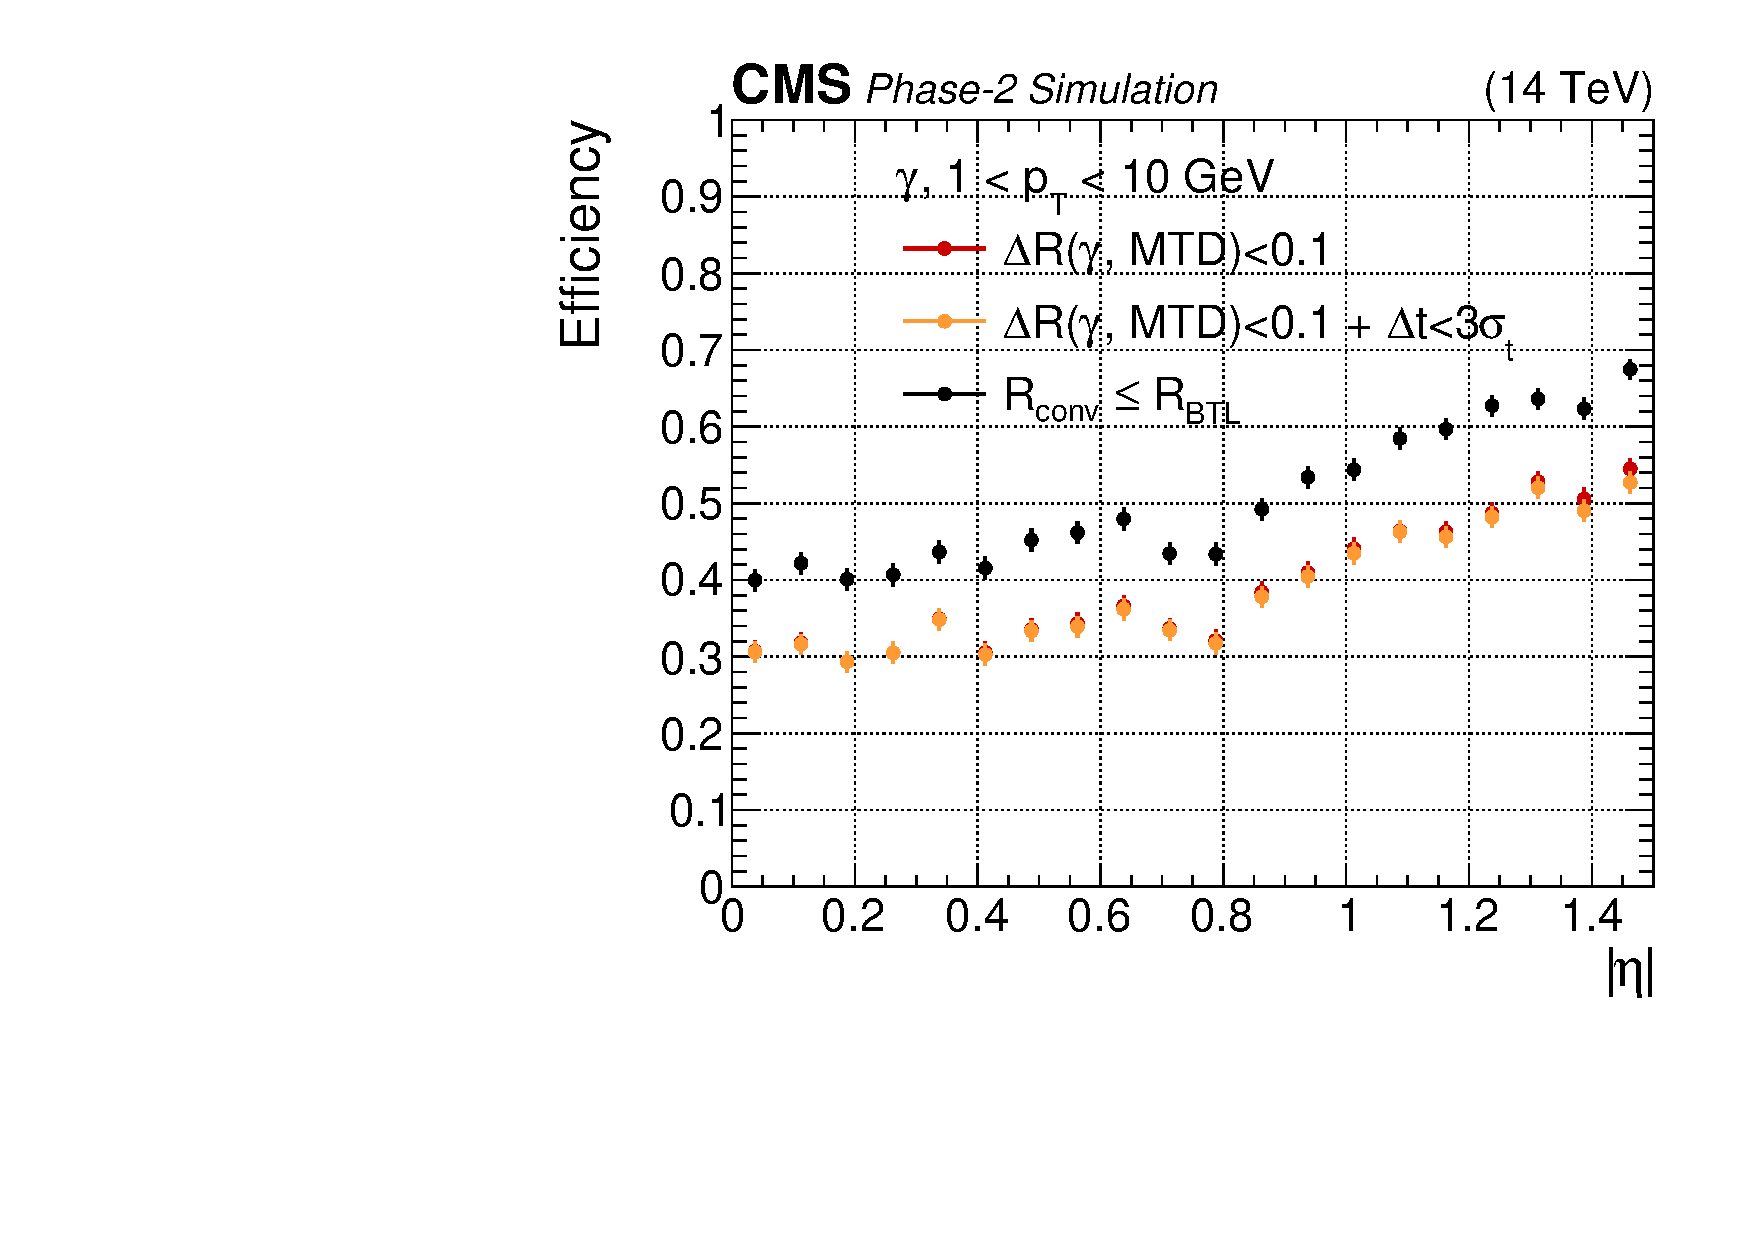
\includegraphics[width=0.48\textwidth]{fig/performance/neutrals/neutrals_efficiency_vs_eta.pdf}
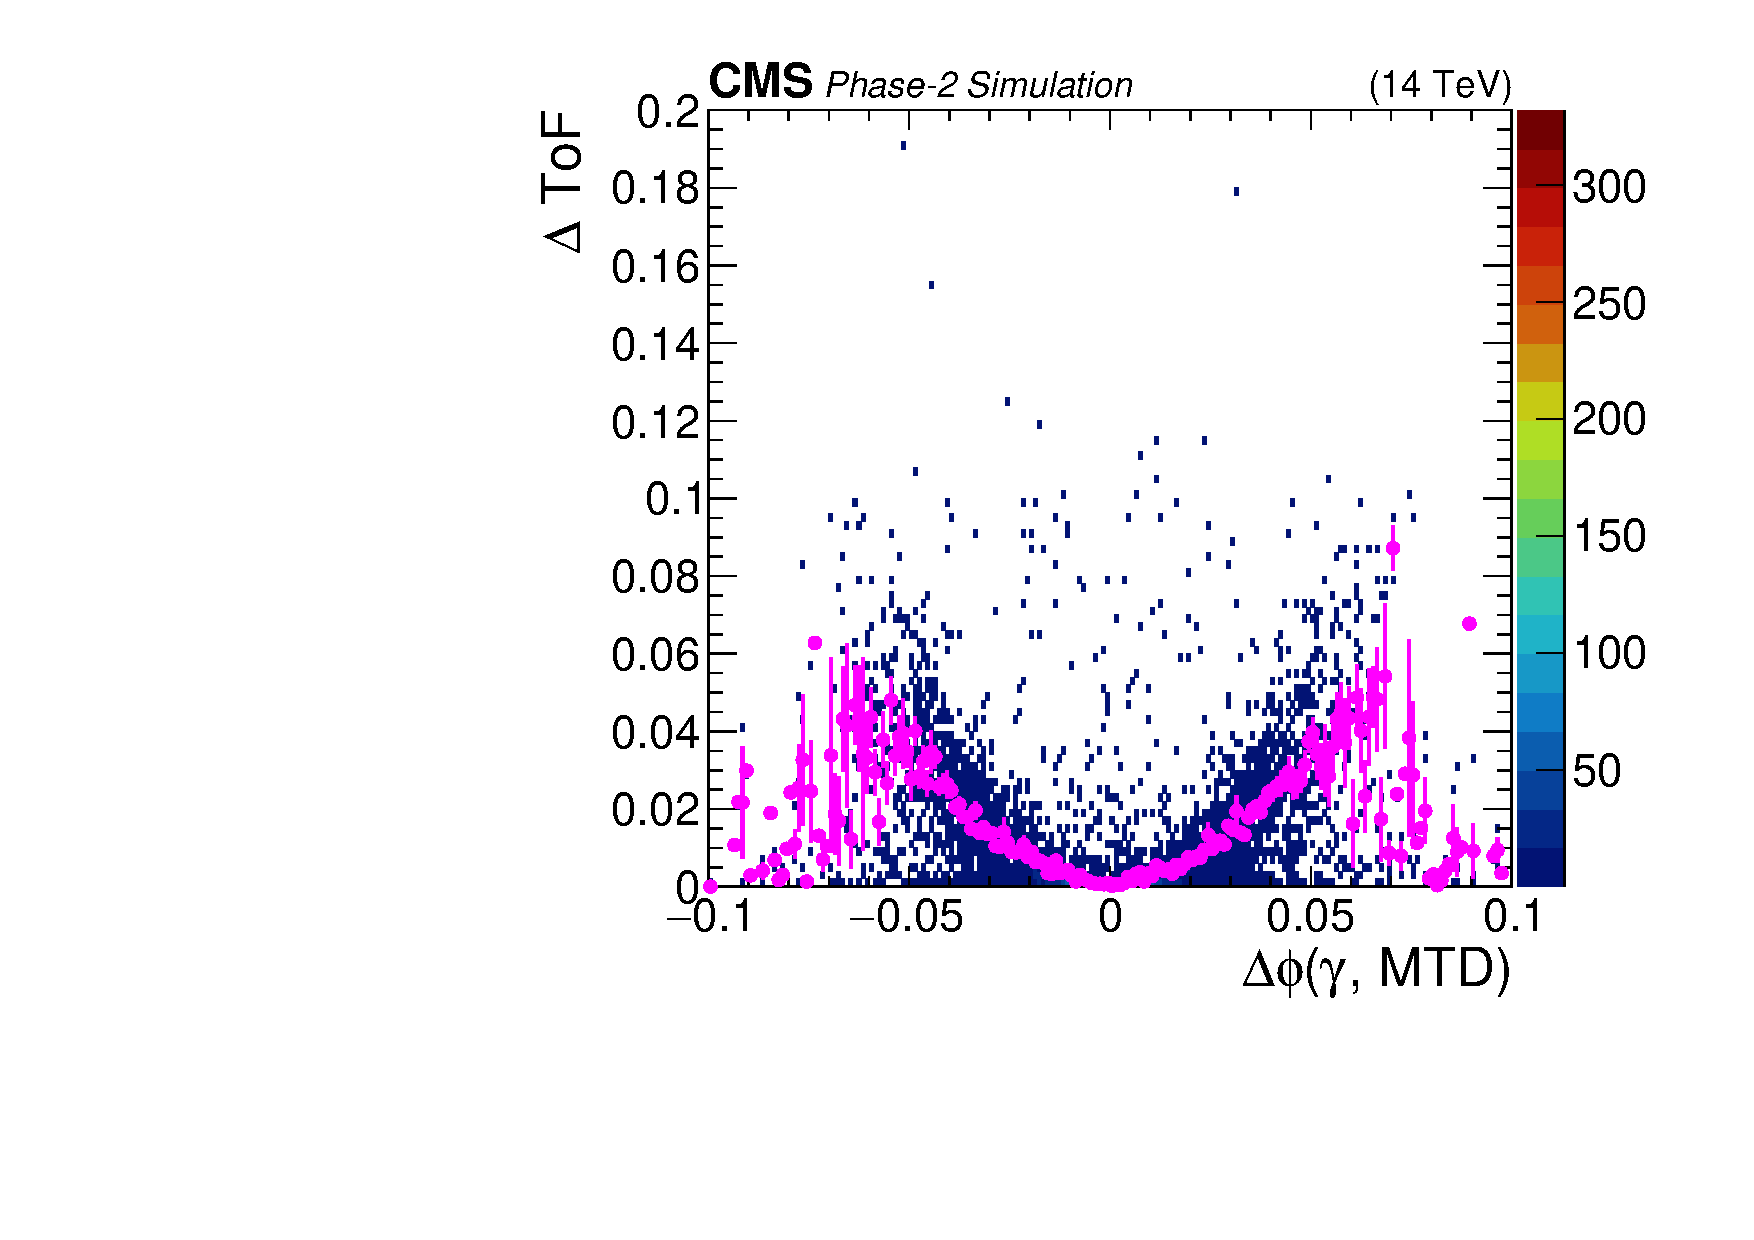
\includegraphics[width=0.48\textwidth]{fig/performance/neutrals/delta_tof_vs_dPhi.pdf}
\caption{(left) Probability to have a conversion within the BTL radius as a function of pseudo-rapidity. (right) Correction to the time-of-flight obtained as the difference between the simulated hit time and the time to travel the (MTD-vertex) distance. The correction is parametrised as a function of $\Delta\phi(ECAL,MTD)$.}
\label{fig:neutrals_mustache}
\end{figure}

$\chi^{2}$ compatibility criteria can then be derived both for the time and space coordinates as discussed for the track-MTD association knowing the vertex time.  $\chi^2=\chi^2_{space}+W\times\chi^2_{time}$, weighting with a factor of 5 more the time compatibility, is used to sort the hits and choose the most compatible MTD hit. Time is weighted more than position since for low $p_{T}$ conversion MTD hits can be found significantly displaced in the $\phi$ coordinate from the propagated ECAL position. For simplicity, no information is currently used from the conversion tracks even when these are reconstructed; this can be improved in the future. As discussed for the track association, in absence of the vertex time the beam spot parameters can also be used to derive the constraint.

%\begin{equation}
%\end{equation}

%%PM Add a plot of chi2?

In order to define a proper association between an ECAL cluster and an MTD cluster $\chi^{2}_{time}<5$ and  $\chi^{2}_{space}<50$ are required.
The efficiency to assign time to a PFCandidate is reported as a function of the $\eta$ coordinate (left) and of the the generated photon $p_{T}$ (right) in Fig.\ref{fig:neu_eff_PU0}. Single photon events with a flat $p_{T}$ spectrum between 1 and 10 GeV and without pile-up are used. The PFCandidates are required to be within $\Delta R<0.5$ from the generated photon (for a single generated photon more than one PFCandidate can be matched when the conversion happens early enough) and to have reconstructed $p_{T}>1$~GeV. 
The probability to have a conversion within the BTL radius is reported in black as the ultimate reachable absolute efficiency. The absolute time reconstruction efficiency for a neutral PFCandidate goes from ~30\% at the begin of the BTL to nearly 50\% at the end of the BTL. This efficiency accounts for the conversion probability within the BTL volume and the reconstruction efficiency which is about 80\%. The loss of reconstruction efficiency is mostly due to the BTL geometric efficiency and for a small fraction also to the late conversions in the LYSO crystals, which produce hits below the energy threshold of 1 MeV.

\begin{figure}[!hbtp]
\centering
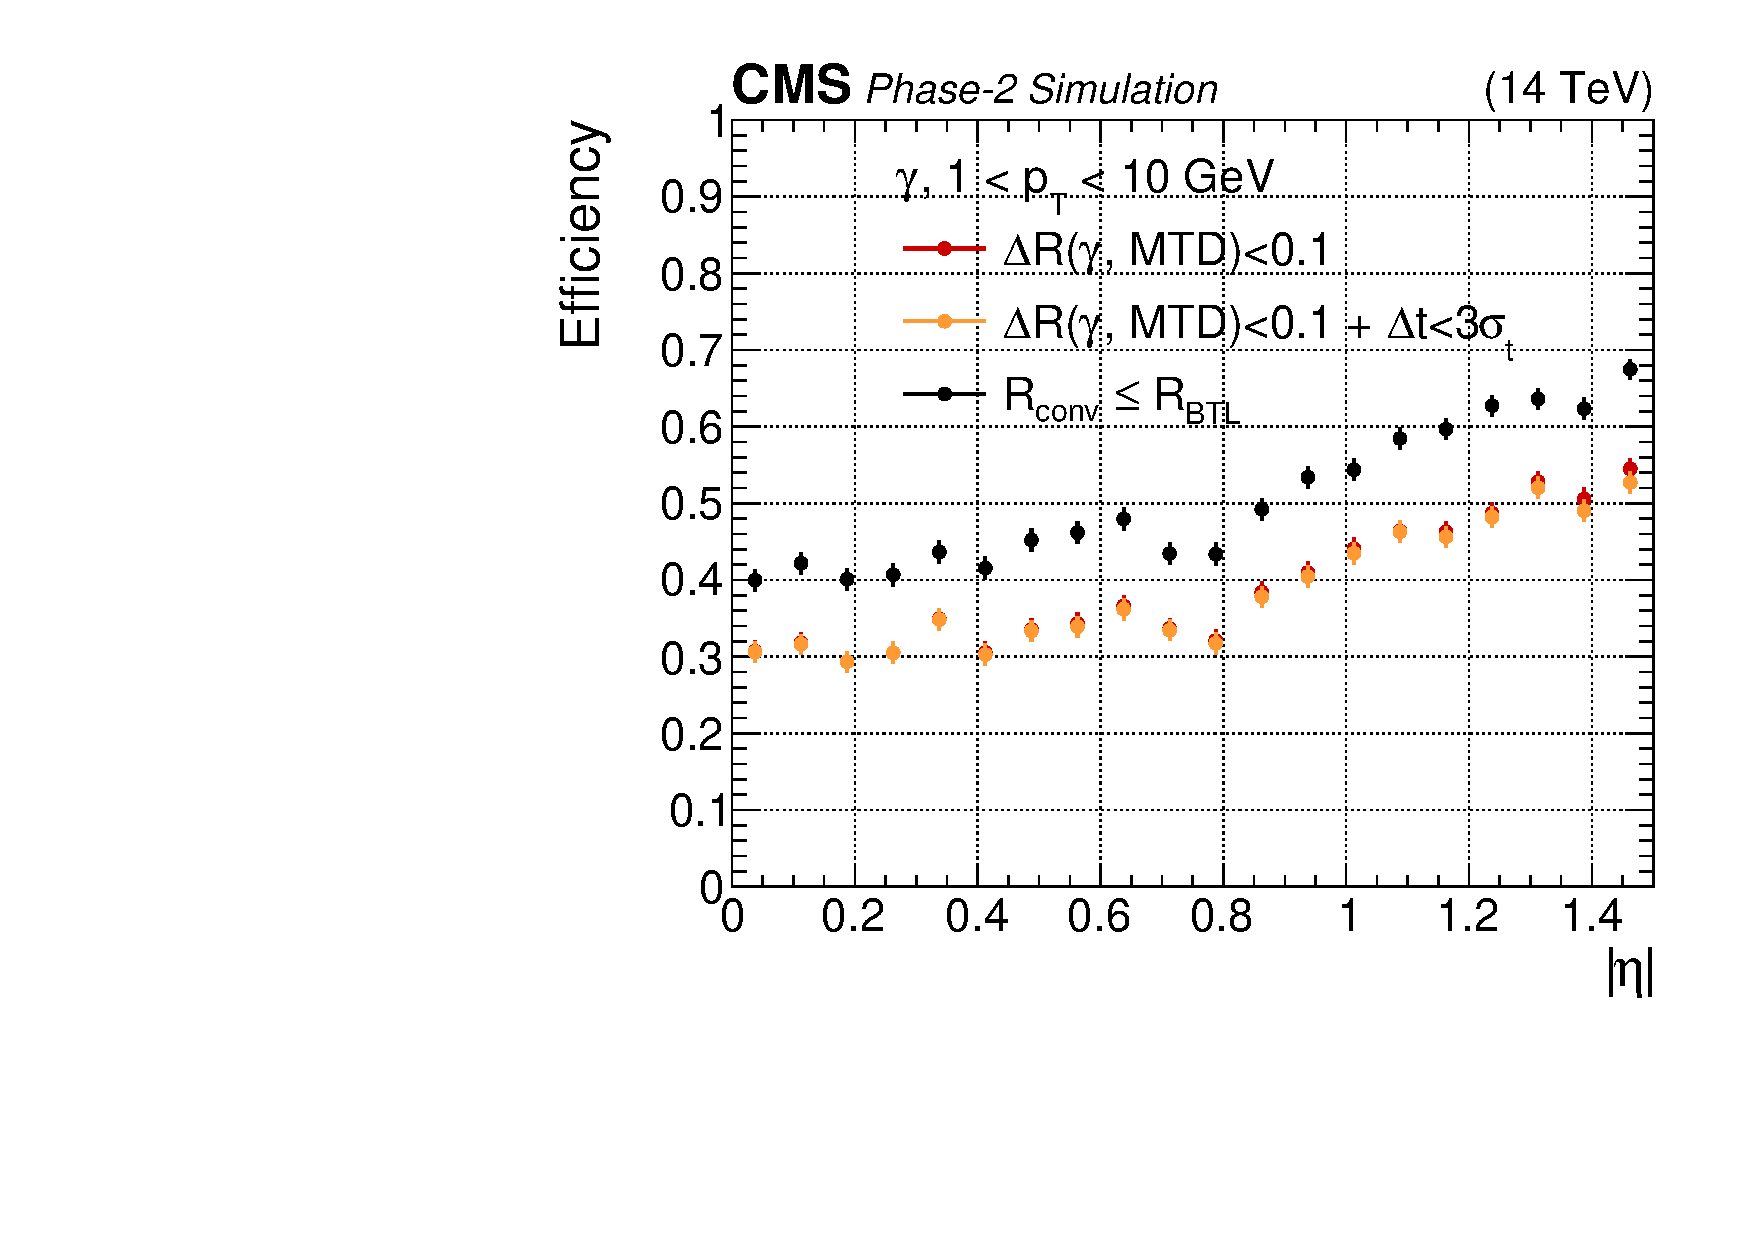
\includegraphics[width=0.48\textwidth]{fig/performance/neutrals/neutrals_efficiency_vs_eta.pdf}
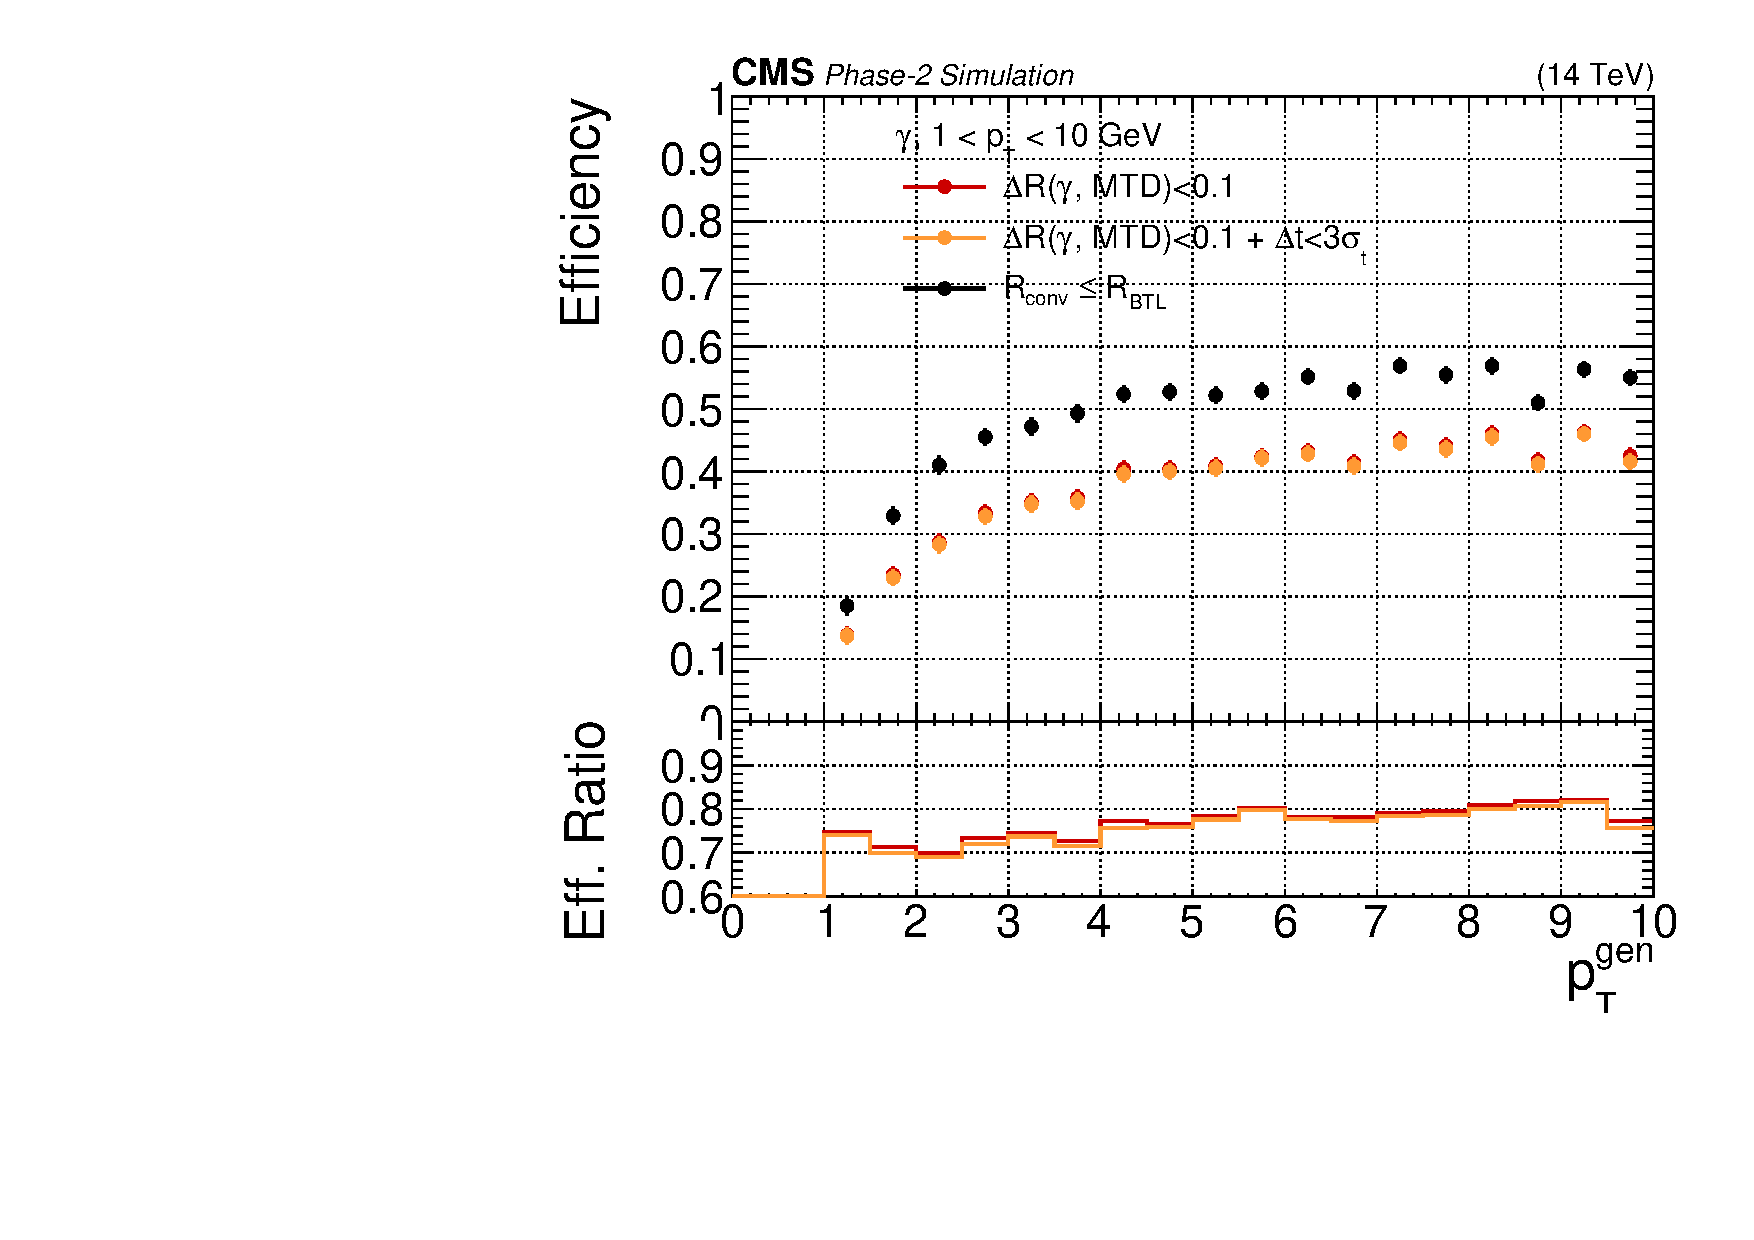
\includegraphics[width=0.48\textwidth]{fig/performance/neutrals/neutrals_efficiency_vs_genPt_minDR0p1.pdf}
\caption{Probability to find an associated BTL cluster for a neutral PFCandidate as a function of pseudo-rapidity (left) and generated photon $p_{T}$ (right). Single photon events with a flat $p_{T}$ spectrum between 1 and 10 GeV and without pile-up are used. The PFCandidates are required to be within $\Delta R<0.5$ from the generated photon and to have reconstructed $p_{T}>1$~GeV. Black corresponds to the probability to have a conversion within the BTL radius, red is the probability to find an MTD cluster, orange is further requiring that the associated time to be within $3\sigma$ of the generated vertex time.}
\label{fig:neu_eff_PU0}
\end{figure}

The time resolution for events without pile-up is reported in \ref{fig:neu_tres} (left). The resolution is 32ps, very similar what has been reported for charged particles, showing that the impact from the path length to the time-of-flight back-propagation is negligible compared to the BTL intrinsic time resolution. The improvement with respect to the charged particles time resolution is due to the slightly larger average deposited energy. The resolution is also computed at PU200 \ref{fig:neu_tres} (right), showing a negligible degradation and demonstrating that also in the high pile-up environment it will be possible to reconstruct time for low energy EM deposits. The efficiency as a function of $\eta$ has been computed also at PU200 in Fig.\ref{fig:neu_eff_PU0} showing a small degradation of performance, also partially due to deterioration of the ECAL reconstruction from pile-up noise. In these early studies, we have not yet tried to improve the ECAL reconstruction using MTD informations, which is left as a subject for future studies. Also further improvements in the future can be achieved combining the time as measured from ECAL with the MTD time reconstruction.

\begin{figure}[!hbtp]
\centering
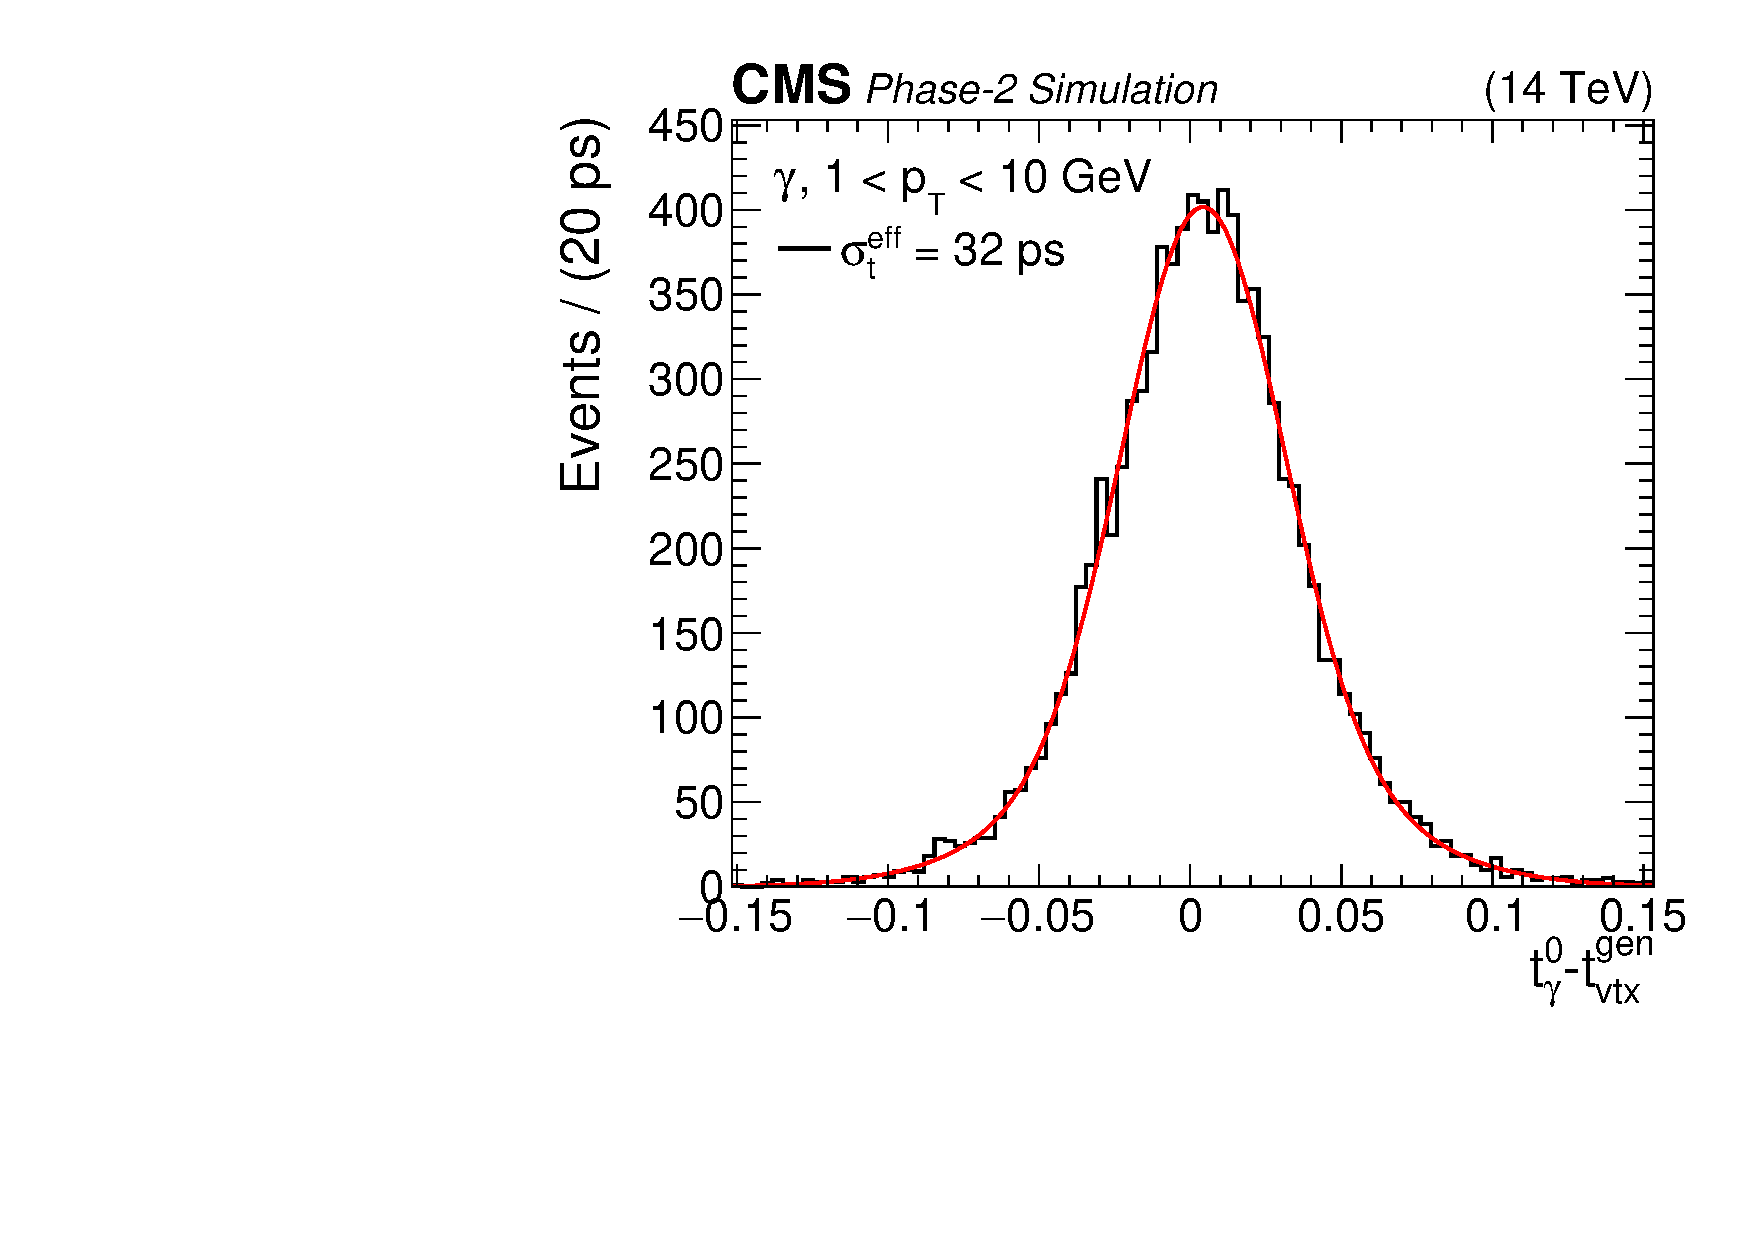
\includegraphics[width=0.48\textwidth]{fig/performance/neutrals/t0_resolution_simhtof.pdf}
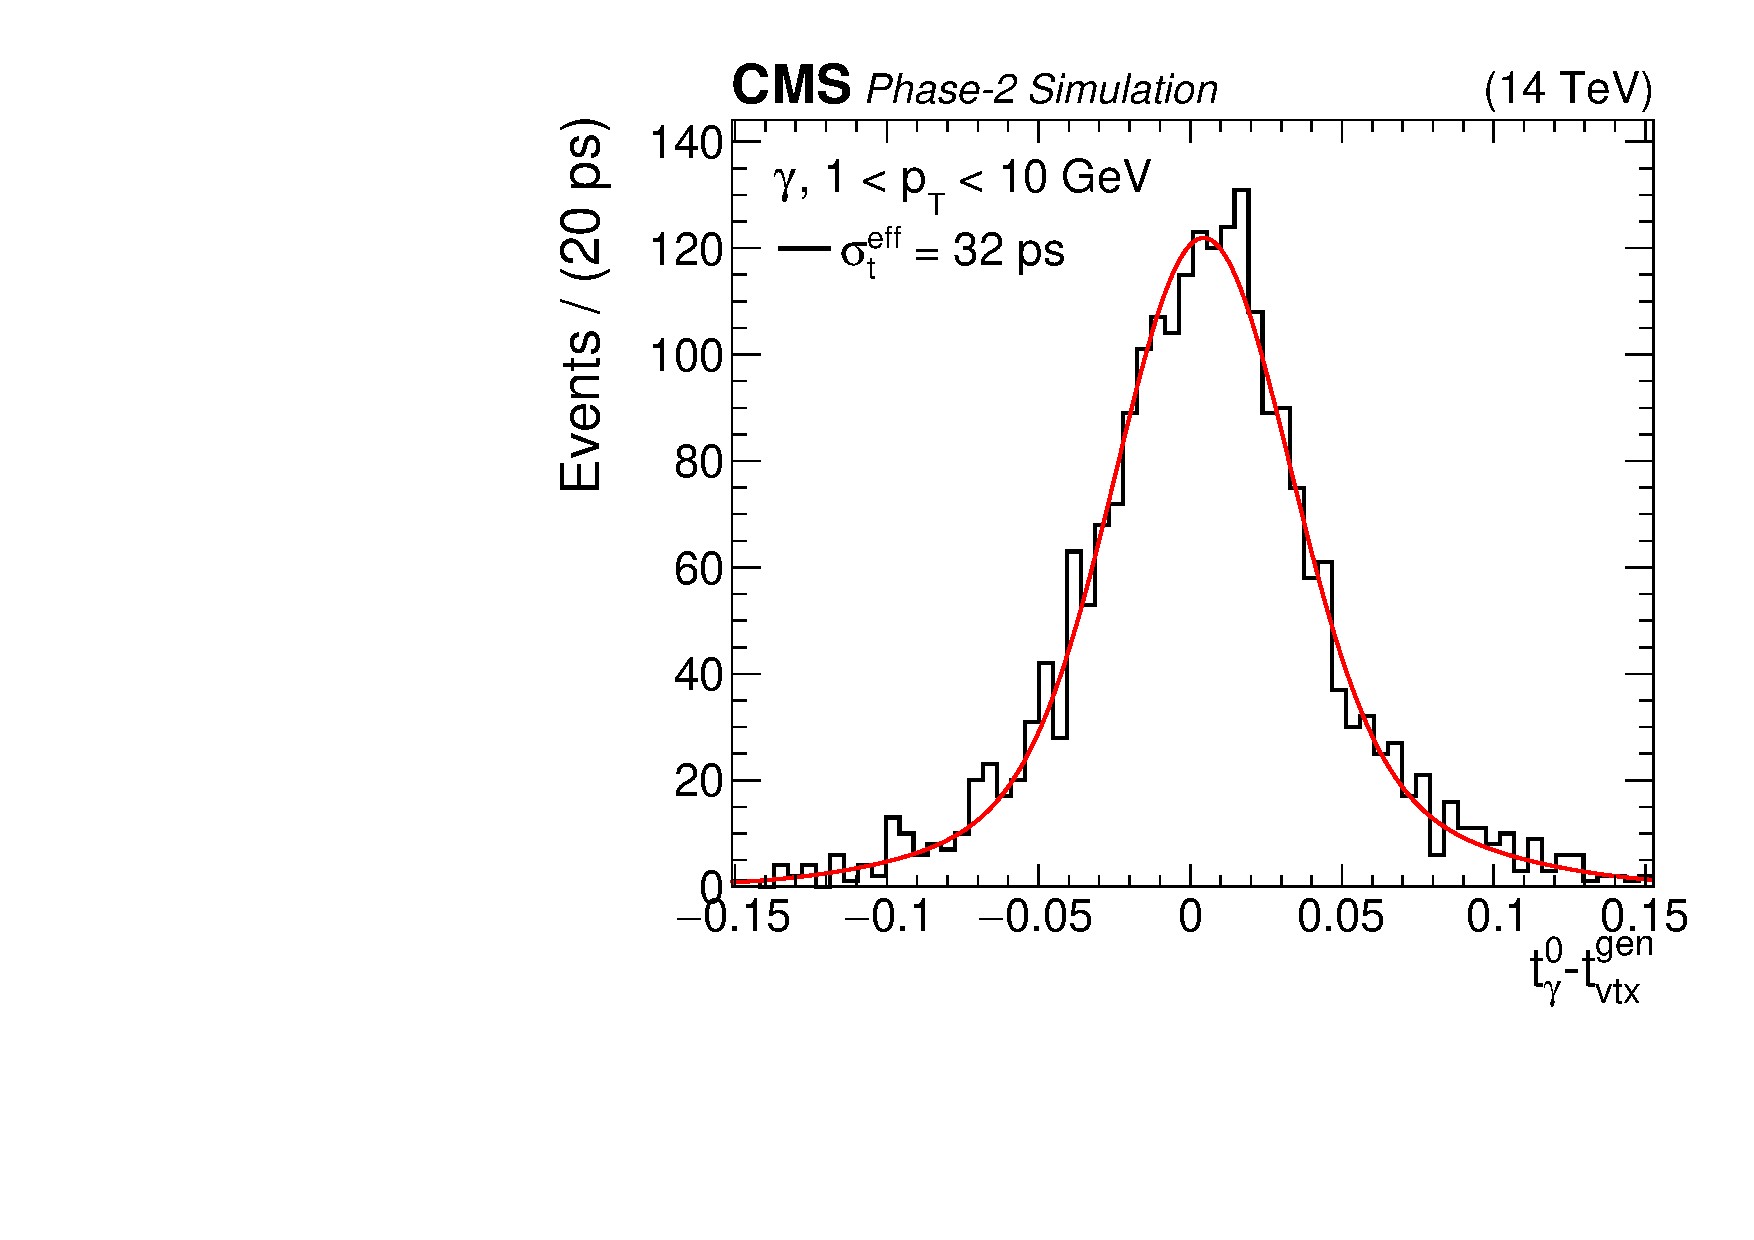
\includegraphics[width=0.48\textwidth]{fig/performance/neutrals/t0_resolution_simhtof-200PU.pdf}
\caption{Reconstructed time for neutral particles in BTL confronted to the vertex time. (left) PU0 conditions, (right) PU200. Single photon events with $1<p_{T}<10$~GeV are used. Effective time resolution is 32ps for PU0 conditions and 35ps for PU200.}
\label{fig:neu_tres}
\end{figure}
